\section{Changing integration variables}
\lecture{12}{6/2}

In general, a map from one coordinate to another should be a
\emph{diffeomorphism} (that is, differentiable and invertible).

\begin{example}
    Consider changing from $(r, \theta)$ to $(x,y)$ (and back).
    We have
    \[
        \bm v(r, \theta) =
        \begin{pmatrix}
            x(r,\theta) \\
            y(r,\theta) \\
        \end{pmatrix}
        =
        \begin{pmatrix}
            r\cos\theta \\
            r\sin\theta \\
        \end{pmatrix}
        .
    \]
    Suppose we have an area integral of $f(x,y)$ over the
    region $V \subset \R^2$
    On the cartesian side
    \[
        I = \int_V f(x,y) \,dx\,dy.
    \]
    In terms of polars, we have 
    $(x,y) = \bm v(r, \theta) = (r\cos\theta, r\sin\theta)$
    and $(x,y) \in V \implies (r,\theta) \in U$
    where $V = \bm v(U)$.
    Our aim is to rewrite $I$ in terms of $r$ and $\theta$.
    We do this by adapting our more general formula for surface
    integrals, considering $(r, \theta)$ as a parametrisation
    for the region $V$ with $U$ as the appropriate parameter domain.
    We embedd everything in $\R^3$ to do this.
    Let
    \[
        S = \{ (x,y,z)\in\R^3: (x,y) \in V, z = 0 \}
    \]
    with unit normal $\bm e_3$.
    We set
    \[
        \bm F(x,y,z) = (0,0,f(x,y)).
    \]
    Then
    \[
        I = \int_V f(x,y) \,dx\,dy = \int_S \bm F \cdot d\bm A.
    \]
    In general, we parametrise $S$ by $(u,v)$ using $\bm x = \bm x(u,v)$.
    \[
        \int_S \bm F \cdot d\bm A = \int_U \bm F \cdot
        \left(
            \frac{\partial \bm x}{\partial r} 
            \times
            \frac{\partial \bm x}{\partial \theta} 
        \right)
        \,dr\,d\theta
    \]
    but
    \begin{align*}
        \frac{\partial \bm x}{\partial r}
        \times
        \frac{\partial \bm x}{\partial \theta}
        &= (x_r, y_r, 0) \times (x_\theta, y_\theta, 0) \\
        &=
        \begin{vmatrix}
            \bm e_1 & \bm e_2 & \bm e_3 \\
            x_r & y_r & 0 \\
            x_\theta & y_\theta & 0 \\
        \end{vmatrix}
        \\
        &= \bm e_3(x_ry_\theta - x_\theta y_r) \\
        &= J(\bm v)\bm e_3
    \end{align*}
    so
    \[
        I = \int_U f(r,\theta) J(\bm v) \,dr\,d\theta. \tag{$\star$}
    \]
\end{example}

\begin{remark}
    $(\star)$ generalises to any $\bm v$ in any number of dimensions, but
    we do need a modulus:
    \[
        I = \int_U f(u,v) \abs{J(\bm v)} \,du\,dv
    \]
    (or any $du\,dv\,dw$ and others).
\end{remark}

\begin{figure}[]
    \centering
    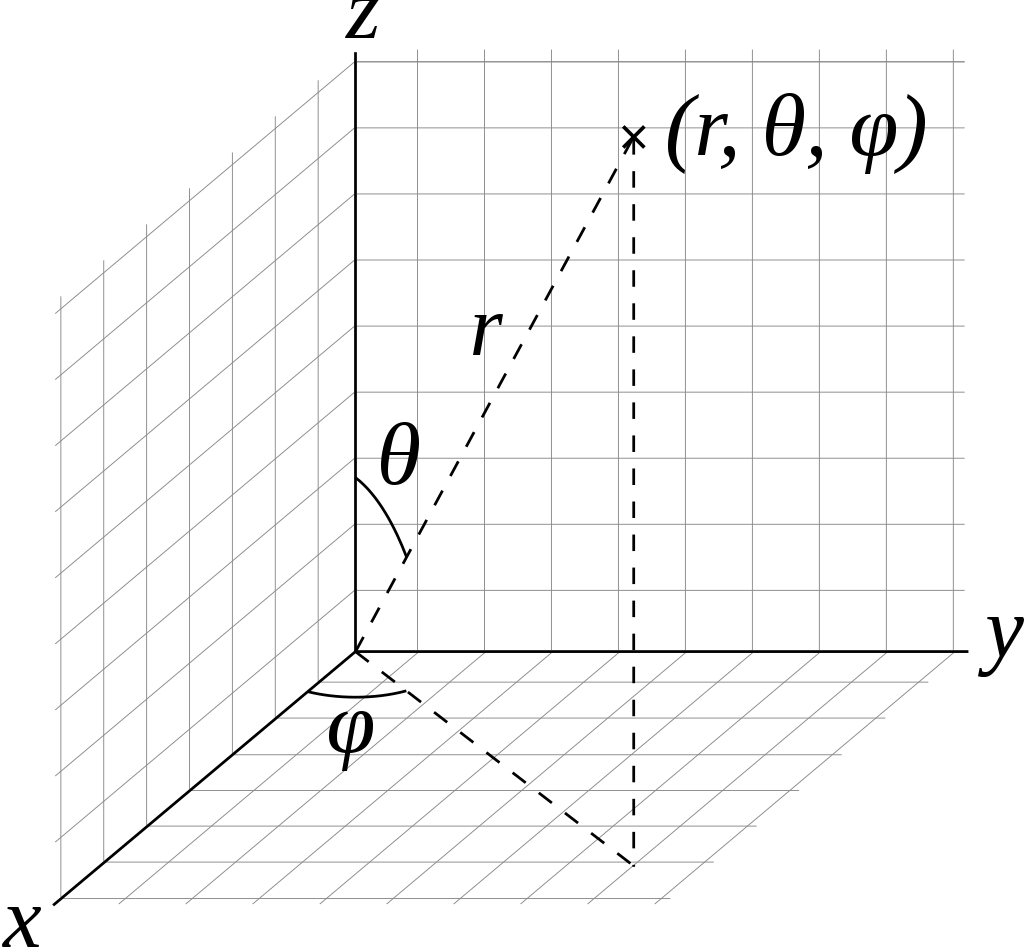
\includegraphics[width=0.8\linewidth]{images/spherical-coordinates.png}
    \caption{A diagram showing spherical coordinates.}%
    \label{fig:spherical-coordinates}
\end{figure}

\begin{example}[Spherical coordinates]
    Here
    \[
        \bm x(r,\theta,\varphi)=
        \begin{pmatrix}
            r\sin\theta\cos\varphi \\
            r\sin\theta\sin\varphi \\
            r\cos\theta \\
        \end{pmatrix}.
    \]
    So
    \[
        \int_V f(x,y,z) \,dx\,dy\,dz
        = \int_U f(r,\theta,\phi) r^2\sin\theta \,dr\,d\theta\,d\varphi.
    \]
    Let's just do a check.
    \begin{align*}
        V &= \{(x,y,z) \in \R^3: \sqrt{x^2 + y^2 + z^2} \leq R\} \\
        U &= \{
                (r,\theta,\varphi) \in \R^3: r \in [0,R],
                                             \theta \in [0,\pi],
                                             \varphi \in [0,2\pi]
             \} \\
        \int_V 1 \,dx\,dy\,dz
        &= \int_U 1 c\dot r^2\sin\theta \,dr\,d\theta\,d\varphi \\
        &= \int_0^{2\pi} \int_0^\pi \int_0^R
            r^2 \sin\theta \,dr\,d\theta\,d\varphi \\
        &= \int_0^{2\pi} \int_0^\pi \frac{R^3}{3} \sin\theta
            \,d\theta\,d\varphi \\
        &= \frac{R^3}{3} \int_0^{2\pi} (-\cos\theta)^\pi_0 \,d\varphi \\
        &= \frac{R^3}{3} \int_0^{2\pi} (2) \,d\varphi \\
        &= \frac{2R^3}{3} (2\pi) \\
        &= \frac{4\pi R^3}{3}.
    \end{align*}
\end{example}

\begin{example}
    Integrate $f(x,y) = x^2 + y^2$ over $V$
    where $V$ is the square with vertices
    \[
        (0,0), \qquad (1,1) \qquad (2,0), \qquad (1,-1).
    \]
    For $(x,y)$, the limits are messy. 
    Instead, we can switch coordinate systems using $u = x + y$
    and $v = x - y$.
    Then $(x,y) \in V \iff u,v \in [0,2]$
    and also
    \[
        x = \frac{1}{2} (u + v), \qquad y = \frac12 (u - v).
    \]
    So
    \[
        \abs{J} = \abs{
            \begin{vmatrix}
                x_u & x_v \\
                y_u & y_v \\
            \end{vmatrix}
        }
        = \abs{
            \begin{vmatrix}
                \frac12 & \frac12 \\
                \frac12 & -\frac12 \\
            \end{vmatrix}
        }
        = \abs{-\frac12} = \frac12.
    \]
    So $x^2 + y^2 = \frac12(u^2 + v^2)$.
    Hence
    \begin{align*}
        I
        &= \int_U \frac12(u^2 + v^2) \frac12 \,du\,dv \\
        &= \int_0^2 \int_0^2 \frac14 (u^2 + v^2) \,du\,dv \\
        &= \frac12 \int_0^2\int_0^2 u^2 \,du\,dv \\
        &= \frac12 \int_0^2 \left(\frac{u^3}3\right)^2_0 \,dv \\
        &= \frac12 \int_0^2 \frac83 \,dv \\
        &= \frac83.
    \end{align*}
\end{example}
